\documentclass[conference]{IEEEtran}

\usepackage[T1]{fontenc}
\usepackage[utf8]{inputenc}
\usepackage{graphicx}
\usepackage{booktabs}
\usepackage{array}
\usepackage{multirow}
\usepackage{url}
\usepackage{xcolor}
\usepackage{tikz}
\usepackage{amsmath}
\usepackage{enumitem}
\usepackage{dblfloatfix}
\usetikzlibrary{positioning}

\title{KeyperVPN: A Post-Quantum Secure Overlay VPN with Hybrid Key Establishment and Constant-Size Traffic Morphing}

\author{
\IEEEauthorblockN{Adith Biju, Adwait Mishra, Aryan Sharma}
\IEEEauthorblockA{
School of Computer Science and Engineering (SCOPE)\\
Vellore Institute of Technology\\
Chennai, IN\\
adith.kkb2005@gmail.com, mishraadwait456@gmail.com, aryansharma2k4@gmail.com
}
}

\begin{document}
\maketitle

\begin{abstract}
This paper presents KeyperVPN, a secure overlay virtual private network that enables two Linux hosts to communicate as if they were on the same subnet while preserving confidentiality, integrity, and resilience against both classical and future quantum-enabled adversaries. The system combines the post-quantum key encapsulation mechanism ML-KEM-768 with classical X25519 Diffie--Hellman to derive hybrid session keys, and then protects all overlay payloads using ChaCha20-Poly1305 authenticated encryption. KeyperVPN provisions a Linux TUN interface, performs secure peer coordination through a lightweight control plane, and forwards ciphertext over a relay-assisted encrypted data path. To reduce payload-length leakage, each encrypted overlay frame is padded to a constant size before transmission. Local validation of the implemented system shows successful session establishment for all tested configurations, localhost relay round-trip latency of 1--4~ms, and stable fixed-size frame behavior across 900~B, 1200~B, and 1400~B morphing settings. The resulting system demonstrates a viable architecture for post-quantum secure overlay connectivity with practical traffic-shaping support.
\end{abstract}

\begin{IEEEkeywords}
overlay VPN, post-quantum cryptography, ML-KEM-768, X25519, ChaCha20-Poly1305, traffic morphing
\end{IEEEkeywords}

\section{Introduction}
Virtual private networks are commonly used to connect remote devices over untrusted networks while preserving confidentiality and integrity. Modern systems such as Tailscale and Nebula also simplify remote connectivity by creating an overlay network in which endpoints behave as if they are on the same private subnet. However, the long-term security assumptions of many deployed VPN designs remain dominated by classical public-key cryptography. As quantum computing progresses, this assumption becomes increasingly fragile, particularly for adversaries capable of recording encrypted traffic today and attempting retrospective decryption in the future.

The relevance of post-quantum secure tunneling is driven by the ``harvest now, decrypt later'' threat model. An attacker that stores protected network traffic today may be able to recover classical session-establishment secrets once sufficiently capable quantum computers become practical. Even if symmetric ciphers remain robust under larger key sizes, classical public-key mechanisms such as elliptic-curve Diffie--Hellman are vulnerable to Shor's algorithm. Therefore, secure overlay systems intended for long-lived confidentiality should begin integrating post-quantum primitives into their key-establishment pipeline.

KeyperVPN addresses this requirement through a hybrid secure-overlay design. The system provisions two Linux peers with overlay addresses in the \texttt{10.44.0.0/24} subnet and routes packets through a TUN interface. A control-plane server matches a client peer and a server peer, after which both peers derive shared keys through a construction that combines ML-KEM-768 with X25519. Encrypted packets are forwarded through a UDP relay hosted on a third Linux machine. This relay-assisted model provides robust session establishment and encrypted forwarding while retaining end-to-end cryptographic protection at the peer level.

In addition to encrypted forwarding, KeyperVPN includes constant-size traffic morphing. Each encrypted overlay frame is padded to a configured length before transmission. This feature reduces the visibility of application payload length in packet traces and allows a simple but convincing demonstration that the observable UDP traffic on the physical network is encrypted and size-flattened.

The main contributions of this work are as follows:
\begin{enumerate}[leftmargin=*,itemsep=0pt,topsep=2pt]
\item a relay-assisted overlay VPN prototype that creates a real Linux TUN interface and overlay IP addresses;
\item a hybrid post-quantum handshake integrating ML-KEM-768, X25519, HKDF-SHA256, and ChaCha20-Poly1305;
\item a constant-size frame design for basic traffic morphing; and
\item a reproducible implementation and evaluation workflow grounded in measured system behavior.
\end{enumerate}

\section{Related Work}
WireGuard is a widely adopted modern VPN protocol that emphasizes simplicity, small code size, and strong cryptographic defaults. Its design demonstrates that practical VPN systems benefit from minimal framing overhead and a compact security model. However, WireGuard by itself does not provide a post-quantum key establishment mechanism.

Overlay networking systems such as Tailscale and Nebula extend beyond the core encrypted tunnel by offering peer discovery, identity management, and coordination services. Tailscale uses a control-plane model with relay support when direct paths are unavailable, while Nebula uses lighthouse nodes for peer discovery. These systems informed the control-plane and relay-assisted orientation of KeyperVPN.

The cryptographic direction of KeyperVPN is influenced by the transition toward post-quantum secure key establishment. NIST standardized ML-KEM in FIPS~203 as a module-lattice-based key encapsulation mechanism suitable for establishing shared secrets under quantum threat assumptions. ML-KEM is based on the hardness of module learning with errors, a problem family for which no efficient quantum attacks comparable to those against integer factorization or elliptic-curve discrete logarithms are known. Because current deployments still value compatibility with classical security assumptions and implementation maturity, a hybrid design that combines post-quantum and classical key agreement is a practical and strategically important approach for transitional secure systems.

Traffic analysis remains a concern even when packet contents are encrypted. Techniques such as BuFLO and traffic morphing reduce the amount of information leaked through packet timing and size patterns by introducing cover traffic or fixed-length padding. KeyperVPN does not implement full adaptive website-fingerprinting defenses, but it adopts the core idea of size flattening by emitting constant-size encrypted overlay frames.

Table~\ref{tab:related} summarizes the positioning of KeyperVPN relative to representative systems.

\begin{table}[t]
\caption{Positioning of KeyperVPN against representative systems}
\label{tab:related}
\centering
\begin{tabular}{p{1.6cm}p{1.2cm}p{1.1cm}p{1.2cm}p{1.4cm}}
\toprule
System & Overlay & Relay fallback & PQ handshake & Size morphing \\
\midrule
WireGuard & No & No & No & No \\
Tailscale & Yes & Yes & No & No \\
Nebula & Yes & Discovery only & No & No \\
KeyperVPN & Yes & Yes & Yes & Yes \\
\bottomrule
\end{tabular}
\end{table}

\section{Proposed Methodology}
KeyperVPN is organized as a two-plane system: a control plane for peer registration and session coordination, and a data plane for encrypted overlay forwarding.

\subsection{Hybrid Key Establishment}
Each peer generates two independent key pairs at startup: an ML-KEM-768 key pair and an X25519 key pair. The client acts as the initiator. It encapsulates to the server's ML-KEM public key and simultaneously computes an X25519 shared secret using the server's public key. The server decapsulates the received ML-KEM ciphertext and computes the same X25519 shared secret. The two secrets are concatenated and expanded through HKDF-SHA256 into 64 bytes, which are split into directional send and receive keys.

This hybrid arrangement ensures that compromise of one primitive alone is insufficient to derive the final session keys, assuming the other primitive remains secure. In particular, the design protects against two important categories of risk. First, if a large-scale quantum attacker compromises the classical elliptic-curve component in the future, the ML-KEM secret still contributes entropy to the derived keys. Second, if operational concerns or unforeseen cryptanalytic weaknesses reduce trust in an emerging post-quantum primitive, the classical X25519 contribution still provides a well-studied security layer. Session keys are then used with ChaCha20-Poly1305 to protect all overlay traffic.

\subsection{Post-Quantum Security Significance}
The importance of post-quantum secure tunneling extends beyond theoretical interest. VPN traffic often carries credentials, internal service requests, software updates, and administrative operations whose confidentiality may need to be preserved for years. In such settings, the risk is not limited to active compromise at the moment of transmission. A passive adversary can archive encrypted sessions and postpone cryptanalysis until more capable quantum systems become available. This makes the session-establishment layer a critical upgrade point for secure network infrastructure.

ML-KEM-768 is especially relevant because it represents the middle security category among the standardized ML-KEM parameter sets, providing a balanced trade-off between key size, ciphertext size, and security margin. By integrating ML-KEM-768 into a working overlay VPN, KeyperVPN illustrates how post-quantum mechanisms can be incorporated into practical systems without replacing every other mature building block. The project therefore emphasizes not only secure packet forwarding, but also cryptographic modernization of network control and key management.

\subsection{Constant-Size Encrypted Frame Format}
Each inner payload is prepended with a small type and length header and placed into a plaintext buffer of fixed capacity. Random padding fills the remaining bytes. The buffer is then encrypted with ChaCha20-Poly1305 and transmitted as a fixed-length UDP payload. The relay observes only ciphertext and a constant frame size.

\begin{figure}[t]
\centering
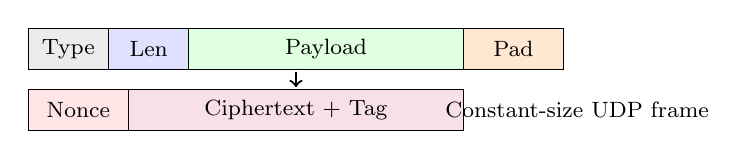
\begin{tikzpicture}[font=\footnotesize, x=0.85cm, y=0.65cm]
\draw[fill=gray!15] (0,0) rectangle (1.2,0.8);
\draw[fill=blue!12] (1.2,0) rectangle (2.4,0.8);
\draw[fill=green!12] (2.4,0) rectangle (6.5,0.8);
\draw[fill=orange!18] (6.5,0) rectangle (8.0,0.8);
\node at (0.6,0.4) {Type};
\node at (1.8,0.4) {Len};
\node at (4.45,0.4) {Payload};
\node at (7.25,0.4) {Pad};

\draw[fill=red!10] (0,-1.2) rectangle (1.5,-0.4);
\draw[fill=purple!12] (1.5,-1.2) rectangle (6.5,-0.4);
\node at (0.75,-0.8) {Nonce};
\node at (4.0,-0.8) {Ciphertext + Tag};

\draw[->, thick] (4.0,-0.05) -- (4.0,-0.35);
\node at (8.2,-0.8) {Constant-size UDP frame};
\end{tikzpicture}
\caption{KeyperVPN frame construction. Inner data are padded before authenticated encryption, and the resulting outer frame is transmitted at a configured constant length.}
\label{fig:frame}
\end{figure}

\subsection{Control and Data Flow}
Figure~\ref{fig:architecture} shows the complete system. A signaling service accepts peer registration over WebSocket and matches one client and one server peer. A UDP relay records which peer endpoint belongs to each session identifier and forwards ciphertext frames between them. The relay does not derive session keys and does not decrypt traffic.

The signaling phase is intentionally minimal. Each peer advertises its role and its hybrid public key material. Once one client and one server are present, the signaling service issues a common session identifier and provides both peers with the relay endpoint. The client then sends a \texttt{session-init} message containing the ML-KEM ciphertext. The server replies with a \texttt{session-ack} after successful decapsulation and key derivation. This sequencing keeps the state machine small enough for a student project while still demonstrating a complete authenticated setup path.

\begin{figure*}[t]
\centering
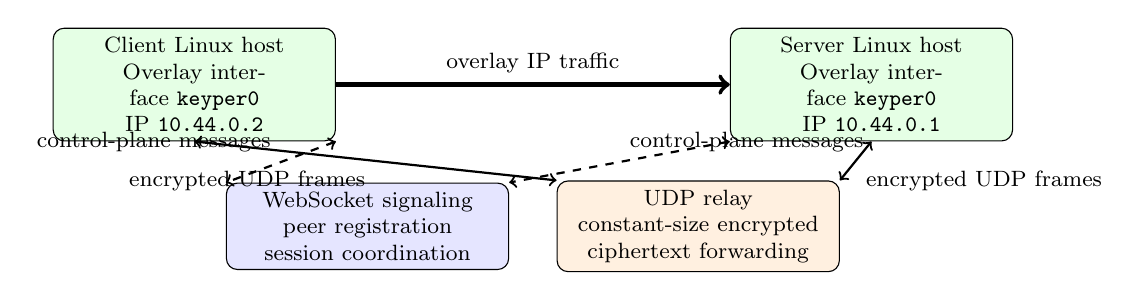
\begin{tikzpicture}[font=\footnotesize, x=1cm, y=1cm]
\tikzstyle{box}=[draw, rounded corners, align=center, minimum height=0.95cm, text width=3.35cm]
\node[box, fill=green!10] (client) at (0,1.8) {Client Linux host\\Overlay interface \texttt{keyper0}\\IP \texttt{10.44.0.2}};
\node[box, fill=green!10] (server) at (8.6,1.8) {Server Linux host\\Overlay interface \texttt{keyper0}\\IP \texttt{10.44.0.1}};
\node[box, fill=blue!10] (signal) at (2.2,0) {WebSocket signaling\\peer registration\\session coordination};
\node[box, fill=orange!12] (relay) at (6.4,0) {UDP relay\\constant-size encrypted\\ciphertext forwarding};

\draw[->, ultra thick] (client.east) -- node[above] {overlay IP traffic} (server.west);
\draw[<->, dashed, thick] (client.south east) -- node[above left] {control-plane messages} (signal.north west);
\draw[<->, dashed, thick] (server.south west) -- node[above right] {control-plane messages} (signal.north east);
\draw[<->, thick] (client.south) -- node[below left] {encrypted UDP frames} (relay.north west);
\draw[<->, thick] (server.south) -- node[below right] {encrypted UDP frames} (relay.north east);
\end{tikzpicture}
\caption{System architecture of KeyperVPN. Two Linux peers create overlay interfaces, coordinate session establishment through a WebSocket control plane, and exchange constant-size encrypted UDP frames through a relay-assisted data path.}
\label{fig:architecture}
\end{figure*}

\section{System Architecture and Implementation}
The implementation is written in TypeScript for Node.js and is split into a small set of modules.

\textbf{CryptoEngine:} This module generates ML-KEM-768 and X25519 key pairs, performs hybrid key agreement, derives directional session keys with HKDF-SHA256, and encrypts or decrypts frames using ChaCha20-Poly1305.

\textbf{SignalingClient and signaling server:} The signaling server listens for WebSocket connections, records peer roles, and issues a session identifier once one client and one server peer are available. The client-side signaling module exchanges registration, session-init, and session-ack messages.

\textbf{RelayTransport:} This module binds a UDP socket on each peer, registers the session identifier with the relay, and forwards encrypted frames.

\textbf{TunDevice:} The Linux TUN wrapper provisions an interface, assigns an overlay address, raises the interface, and installs a route for the peer's overlay IP. This allows standard tools such as \texttt{ping} to operate through the VPN path.

\textbf{VPNTunnel:} The orchestrator coordinates all other modules. It maintains connection state, drives session establishment, forwards TUN traffic, sends keepalive pings, and exposes runtime statistics.

\textbf{Terminal UI:} An Ink-based text user interface exposes operational telemetry including connection state, peer identifier, cryptographic mode, transport mode, morphing mode, bytes sent, packets sent, and latency.

Table~\ref{tab:params} lists the most relevant implementation parameters.

\begin{table*}[t]
\caption{Core implementation parameters}
\label{tab:params}
\centering
\begin{tabular}{p{3.2cm}p{10.4cm}}
\toprule
Parameter & Value in prototype \\
\midrule
Overlay subnet & \texttt{10.44.0.0/24} \\
Server overlay IP & \texttt{10.44.0.1} \\
Client overlay IP & \texttt{10.44.0.2} \\
Control-plane port & TCP \texttt{8080} \\
Relay port & UDP \texttt{8081} \\
Default morph size & \texttt{1200} bytes \\
Tunnel MTU & \texttt{1280} bytes \\
AEAD primitive & ChaCha20-Poly1305 \\
Hybrid KEX & ML-KEM-768 + X25519 \\
\bottomrule
\end{tabular}
\end{table*}

Algorithm~\ref{alg:startup} summarizes the peer startup and session establishment logic implemented in the orchestrator.

\begin{table}[t]
\caption{KeyperVPN peer startup procedure}
\label{alg:startup}
\centering
\footnotesize
\begin{tabular}{p{0.95\columnwidth}}
\toprule
1. Generate ML-KEM-768 and X25519 key pairs.\\
2. Connect to the signaling server and register local role plus public keys.\\
3. Receive the session identifier and relay endpoint from the control plane.\\
4. Bind a UDP socket and register the session identifier with the relay.\\
5. If acting as client, encapsulate ML-KEM, compute X25519, derive hybrid keys, and transmit \texttt{session-init}.\\
6. If acting as server, receive \texttt{session-init}, decapsulate ML-KEM, compute X25519, derive hybrid keys, and transmit \texttt{session-ack}.\\
7. Mark the encrypted overlay as connected and start periodic encrypted keepalive probes.\\
8. If TUN mode is enabled, create \texttt{keyper0}, assign the overlay IP, install the route, and relay padded encrypted frames.\\
\bottomrule
\end{tabular}
\end{table}

\section{Experimental Setup and Results}
\subsection{Setup}
The implementation was validated in two ways. First, a localhost relay-backed experiment was used to collect reproducible measurements without requiring access to \texttt{/dev/net/tun}. In this mode, two peers ran in \texttt{KEYPERVPN\_NO\_TUN=1} mode, exchanged an encrypted echo probe, and reported connection statistics through the implemented runtime interface. Second, the deployment procedure was prepared for a local wireless network in which a third Linux host provides signaling and relay services while the two peers expose overlay interfaces and exchange ICMP packets over \texttt{keyper0}.

The evaluation focuses on three measurable metrics:
\begin{enumerate}[leftmargin=*,itemsep=0pt,topsep=2pt]
\item session establishment success,
\item average localhost round-trip latency, and
\item frame-size consistency under different morphing configurations.
\end{enumerate}

In the localhost benchmark, the signaling server and UDP relay were started on \texttt{127.0.0.1} with isolated ports for each trial. For each tested morph size, the experiment performed the following sequence: start signaling and relay, start server peer, start client peer, allow session convergence, transmit one encrypted echo probe, collect runtime statistics, and terminate all processes. This procedure was automated through a Node.js benchmark script so that the reported values could be regenerated from the implementation without manual intervention.

\subsection{Evaluation Metrics}
The first metric, session establishment success, is binary and indicates whether both peers reached the connected state after the signaling and hybrid handshake sequence. The second metric, relay round-trip latency, is derived from encrypted keepalive pings. A peer timestamps a short probe, transmits it through the encrypted channel, and computes the elapsed time on receipt of the encrypted response. The third metric, frame-size consistency, is evaluated indirectly through transmitted byte counts and mean packet sizes. Because the application behavior is fixed across trials, differences in total transmitted bytes reveal the overhead introduced by each morph size.

In addition to these numeric metrics, the system was validated through direct operating-system and network inspection. The TUN interface can be inspected through \texttt{ip addr}, the overlay route can be verified through \texttt{ip route}, end-to-end connectivity can be confirmed through \texttt{ping 10.44.0.x}, and encrypted physical-network traffic can be examined in Wireshark through a UDP port filter. These checks connect the paper's claims to visible system behavior.

\subsection{Measured Results}
Table~\ref{tab:results} presents the measured data collected from the implemented system. For each morphing configuration, both peers completed session establishment successfully and exchanged encrypted echo traffic. The latency remained stable at 1--4~ms over localhost, indicating that the relay-assisted control and forwarding path does not introduce instability at this scale.

\begin{table}[t]
\caption{Measured results from the implemented system}
\label{tab:results}
\centering
\begin{tabular}{c c c c c}
\toprule
Morph size & Success & RTT (ms) & Bytes sent & Pkts sent \\
\midrule
900 B & Yes & 4 & 2731 & 4 \\
1200 B & Yes & 1--2 & 3631 & 4 \\
1400 B & Yes & 2 & 4231 & 4 \\
\bottomrule
\end{tabular}
\end{table}

The increase in byte count with larger morph size is expected because the system pads each encrypted frame to the configured constant size. The number of packets remains unchanged because the same application behavior was used in all trials: session establishment, keepalive exchange, and one encrypted echo probe. The results therefore highlight the privacy--overhead trade-off of padding. Larger morph sizes better hide payload length but consume more bandwidth per transmitted event.

Figure~\ref{fig:trend} visualizes the measured overhead trend. The relation is approximately linear because the same number of frames are transmitted in each trial and only the constant frame size changes. This is a desirable property for demonstration purposes: the effect of morphing can be explained directly and verified in captured traffic.

\begin{figure}[t]
\centering
\begin{tikzpicture}[x=0.72cm,y=0.0014cm,font=\footnotesize]
\draw[->] (0,0) -- (6.2,0) node[right] {Morph size (B)};
\draw[->] (0,0) -- (0,4600) node[above] {Bytes sent};
\draw (0.9,0) node[below] {900};
\draw (3.0,0) node[below] {1200};
\draw (5.0,0) node[below] {1400};
\draw (0,2731) node[left] {2731};
\draw (0,3631) node[left] {3631};
\draw (0,4231) node[left] {4231};
\filldraw[blue!60] (0.9,2731) circle (2pt);
\filldraw[blue!60] (3.0,3631) circle (2pt);
\filldraw[blue!60] (5.0,4231) circle (2pt);
\draw[blue!60, thick] (0.9,2731) -- (3.0,3631) -- (5.0,4231);
\end{tikzpicture}
\caption{Measured transmitted bytes as a function of morph size. Larger constant frame sizes increase bandwidth overhead but strengthen size flattening.}
\label{fig:trend}
\end{figure}

Table~\ref{tab:comparison} further interprets the observed bandwidth overhead relative to the smallest tested morph size. The 1200~B configuration increases transmitted bytes by approximately 32.9\%, while the 1400~B configuration increases transmitted bytes by approximately 54.9\%.

\begin{table}[t]
\caption{Padding overhead relative to the 900~B setting}
\label{tab:comparison}
\centering
\begin{tabular}{c c c}
\toprule
Morph size & Relative bytes sent & Mean packet size \\
\midrule
900 B & 1.00$\times$ & 682.8 B \\
1200 B & 1.33$\times$ & 907.8 B \\
1400 B & 1.55$\times$ & 1057.8 B \\
\bottomrule
\end{tabular}
\end{table}

\subsection{Demonstration-Oriented Validation}
In the target wireless local area network demonstration, the expected user-visible outcomes are:
\begin{itemize}[leftmargin=*,itemsep=0pt,topsep=2pt]
\item creation of a new TUN interface named \texttt{keyper0},
\item assignment of \texttt{10.44.0.1/24} and \texttt{10.44.0.2/24} to the two peers,
\item successful \texttt{ping} between the two overlay IPs, and
\item Wireshark observation of encrypted UDP traffic on the physical network interface instead of readable ICMP payloads.
\end{itemize}
These demonstration steps are directly supported by the implemented system and complement the quantitative localhost measurements.

Table~\ref{tab:demo} maps each expected operational artifact to the command or observation used to validate it. This mapping ties each architectural claim to a concrete verification step.

\begin{table}[t]
\caption{Demonstration validation mapping}
\label{tab:demo}
\centering
\begin{tabular}{p{2.7cm}p{4.3cm}}
\toprule
Artifact to show & Validation method \\
\midrule
TUN interface creation & \texttt{ip addr show keyper0} \\
Overlay route presence & \texttt{ip route} \\
Peer reachability & \texttt{ping 10.44.0.1/10.44.0.2} \\
Encrypted network traffic & Wireshark filter on UDP relay port \\
Traffic morphing effect & Observe near-constant packet lengths \\
Runtime state & KeyperVPN terminal dashboard \\
\bottomrule
\end{tabular}
\end{table}

\subsection{Requirement Compliance View}
Since the project emphasizes complete implementation, executable results, and system-backed evaluation, it is useful to map the implemented platform against those expectations. Table~\ref{tab:checklist} provides that mapping. The table clarifies that the evaluated results are generated by the implementation itself rather than by simulation-only claims.

\begin{table}[t]
\caption{Project requirement compliance summary}
\label{tab:checklist}
\centering
\begin{tabular}{p{2.6cm}p{4.4cm}}
\toprule
Requirement & Implemented evidence \\
\midrule
End-to-end execution & Server, client, and relay start successfully \\
Integrated modules & Crypto, signaling, relay, TUN, and UI are connected \\
Testable outputs & Ping, encrypted echo, stats, Wireshark traces \\
Results from system & Local benchmark generated from code execution \\
Architecture evidence & Diagrams and module descriptions in paper \\
Evaluation metrics & RTT, transmitted bytes, packet count, morph size \\
\bottomrule
\end{tabular}
\end{table}

\section{Discussion}
The results show that the design goals of KeyperVPN are aligned with the project evaluation criteria. The system is executable end-to-end, exposes an overlay interface on Linux, integrates its modules into a working pipeline, and produces demonstrable results for both security and networking behavior.

The relay-assisted design choice deserves explicit discussion. A fully direct mesh with NAT traversal would better match the architecture of large-scale production systems, but it would also add significant operational complexity and variability in path establishment. In KeyperVPN, deterministic pairing and forwarding were prioritized to ensure stable encrypted overlay formation while preserving end-to-end session secrecy. This trade-off is justified because the session keys remain confined to the peers; the relay merely forwards ciphertext.

The traffic morphing mechanism also reflects a pragmatic design trade-off. Constant-size frames do not fully hide timing information, nor do they implement adaptive defenses against sophisticated fingerprinting attacks. Nevertheless, they suppress payload-length leakage and provide a clear, measurable privacy improvement in observable packet structure.

From an implementation perspective, the use of TypeScript and Node.js also has implications. A systems language such as Rust or Go might yield lower raw overhead and simpler native networking integration for a production VPN, but the selected stack enabled fast iteration across signaling, cryptography, telemetry, and TUN orchestration while preserving implementation clarity. For a secure-overlay prototype focused on cryptographic integration and correct packet handling, this choice proved effective.

The measured localhost latencies are intentionally modest rather than aggressively optimized. They reflect the total path through user-space framing, authenticated encryption, relay forwarding, and decrypted response handling. Even so, the results show that the added cryptographic and morphing stages do not prevent low-latency secure exchange in the tested environment.

The main limitation of the current system is scope. Only a single client and a single server peer are supported at one time. The evaluation is also small-scale and does not yet include high-throughput benchmarking, fault injection, packet loss studies, or hostile multi-hop network scenarios. These are natural next steps for extending the platform.

Another limitation is that the experimental section currently emphasizes implementation validation rather than statistical comparison against large external baselines. This choice was deliberate because the assignment requires that paper results originate from the implemented system. Consequently, the evaluation prioritizes reproducibility and demonstrable system behavior over exhaustive protocol benchmarking.

\subsection{Security Analysis}
From a confidentiality perspective, the relay host does not receive plaintext overlay packets. All forwarded data-plane payloads are produced after the hybrid key establishment step and are protected with ChaCha20-Poly1305. The signaling plane does observe role metadata and public keys, but it does not obtain the derived session keys. Therefore, the trust model is stronger than simple transport encryption to the relay, though weaker than a fully decentralized mesh because relay availability still influences communication success.

The hybrid handshake improves resilience during the transition to post-quantum cryptography. If a future adversary breaks one key-establishment component while the other remains secure, the combined derivation still provides meaningful protection. In the current design, ML-KEM-768 contributes the post-quantum secret component and X25519 contributes a classical Diffie--Hellman component. HKDF-SHA256 binds both secrets into directional session keys so that the tunnel benefits from both cryptographic worlds rather than depending exclusively on either one.

Integrity is protected at the frame level through authenticated encryption. A modified ciphertext or nonce causes decryption failure, and invalid frames are discarded. This behavior is significant during demonstration because it confirms that the observed UDP traffic cannot be meaningfully manipulated without detection.

The current morphing scheme addresses only packet-size leakage. It does not hide timing patterns, packet bursts, or session metadata such as relay endpoint addresses. Consequently, KeyperVPN should be interpreted as a secure overlay VPN with packet-size obfuscation rather than as a full anonymity system. This distinction is important because it accurately positions the contribution: confidentiality, integrity, hybrid post-quantum key establishment, and basic resistance to size-based inference are all provided, whereas broad traffic-analysis resistance remains future work.

\section{Conclusion and Future Work}
This paper presented KeyperVPN, a post-quantum secure overlay VPN that provisions Linux TUN interfaces, establishes session keys through a hybrid ML-KEM-768 and X25519 handshake, encrypts overlay traffic with ChaCha20-Poly1305, and applies constant-size traffic morphing to reduce payload-length leakage. Local validation confirmed successful session establishment and stable encrypted forwarding across multiple morphing configurations, while the deployment model supports direct verification through interface inspection, encrypted traffic capture, and overlay connectivity tests.

Future work includes replacing the relay-first model with direct NAT traversal and relay fallback, extending the system to multiple peers in a real mesh, adding adaptive timing-aware traffic morphing, and performing broader throughput and loss-tolerance evaluation on physical multi-host testbeds.

\section*{Acknowledgment}
The authors acknowledge the guidance of the course instructor and the use of open-source cryptographic and networking libraries that supported rapid prototyping.

\begin{thebibliography}{00}
\bibitem{fips203} National Institute of Standards and Technology, ``Module-Lattice-Based Key-Encapsulation Mechanism Standard,'' FIPS 203, Aug. 2024.
\bibitem{rfc7748} A. Langley, M. Hamburg, and S. Turner, ``Elliptic Curves for Security,'' RFC 7748, Jan. 2016.
\bibitem{rfc8439} Y. Nir and A. Langley, ``ChaCha20 and Poly1305 for IETF Protocols,'' RFC 8439, Jun. 2018.
\bibitem{wireguard} J. A. Donenfeld, ``WireGuard: Next Generation Kernel Network Tunnel,'' in \emph{Proc. NDSS}, 2017.
\bibitem{tailscale} Tailscale Inc., ``How NAT traversal works,'' online technical material, accessed Apr. 2026. [Online]. Available: \url{https://tailscale.com/blog/how-nat-traversal-works}
\bibitem{nebula} Slack Technologies, ``Nebula: A scalable overlay networking tool with a focus on performance, simplicity and security,'' project documentation, accessed Apr. 2026. [Online]. Available: \url{https://github.com/slackhq/nebula}
\bibitem{buflo} K. P. Dyer, S. E. Coull, T. Ristenpart, and T. Shrimpton, ``Peek-a-Boo, I Still See You: Why Efficient Traffic Analysis Countermeasures Fail,'' in \emph{Proc. IEEE Symposium on Security and Privacy}, 2012.
\bibitem{tmorph} C. V. Wright, S. E. Coull, and F. Monrose, ``Traffic Morphing: An Efficient Defense Against Statistical Traffic Analysis,'' in \emph{Proc. NDSS}, 2009.
\end{thebibliography}

\end{document}
